\documentclass[12pt]{article}
\usepackage{listings}
\usepackage{amssymb}
\usepackage{amsthm}
\usepackage{amsmath}
\usepackage{graphicx}
\usepackage{subfig}
\usepackage{multirow}
\usepackage{float}
\usepackage{fancyhdr}
\usepackage{caption, subcaption}
\usepackage{tabularx}
\usepackage{booktabs}
\usepackage{multicol}
\usepackage{array}
\usepackage{adjustbox}
\usepackage[cache=false]{minted}
\usepackage{xcolor}
\usepackage[font=small]{caption}
\usepackage{siunitx}
\usepackage{subfigure}
\usepackage{subcaption}
\usepackage{graphicx} % Include this line in the preamble
\usepackage{pgfplots}
\pgfplotsset{compat=1.17}

\definecolor{bg}{rgb}{1.0, 0.97, 0.7} % Light yellow

\setminted[c]{
  bgcolor=bg,
  linenos,
  fontsize=\footnotesize,
  breaklines
}

\captionsetup{compatibility=false}
\usepackage[hidelinks, colorlinks=true, linkcolor=black, urlcolor=blue, citecolor=red]{hyperref}
%margin settings
\usepackage[left=2.5cm, right=2.5cm, top=4cm, bottom=3cm, footskip=0.5cm]{geometry}
% suppressing page numbers
\renewenvironment{abstract}
{\quotation
  {\large\bfseries\abstractname\centering\par\noindent\rule{\linewidth}{.5pt}\medskip}
  \noindent}
{\par\noindent\rule{\linewidth}{.5pt}\endquotation}

% Make headers
\usepackage{fancyhdr}
\pagestyle{fancy}
\fancyhf{}
\fancyhfoffset[L]{1cm} % left extra length
\fancyhfoffset[R]{1cm} % right extra length
\rhead{Group: 1}
\lhead{HW 06: GPU Accelerated Mandelbrot Function}
\fancyfoot[C]{\thepage}


\lstset{frame=tb,
  language=C,
  aboveskip=3mm,
  belowskip=3mm,
  showstringspaces=false,
  columns=flexible,
  basicstyle={\small\ttfamily},
  numbers=none,
  numberstyle=\tiny\color{red},
  keywordstyle=\color{blue},
  commentstyle=\color{green},
  stringstyle=\color{red},
  breaklines=true,
  breakatwhitespace=true,
  tabsize=3
}
\title{ME 489 Homework 06 \\ GPU Accelerated Mandelbrot Function}
\date{\today}
\author{Enes Çağlar Korkmazgöz 2370567 - Hasan Kaan Özen 2378586}

\begin{document}
\maketitle

\begin{abstract}
In this report, the comparison of serial and GPU accelerator is carried out for a program. This program aims to visualize the mandelbrot set. The "mandelbrot" function in this program calculates the real and imaginary parts for every point in the domain so that iterations can be made to see if the point is part of the mandelbrot set or not. This part of the program is parallelized using CUDA. It is shown that as the grid size increases, the serial method lacks performance and the GPU implementation is superior with 20 to 40 folds in terms of run-time. 
\end{abstract}

\newpage
\tableofcontents
\newpage
\section{Introduction}

\noindent
Parallelization techniques by utilizing the CPU cores/processors is done for multiple cases and it is shown that MPI implementation has a lot of benefits in terms of reduction in spent time. However, development and enhancements in the GPU cores lets us the use of GPU in parallelization of time consuming operations. Although different manufacturers offer different programming languages for their GPU environment, the most accepted GPU language CUDA is used in this study. Initially as the number of cores increases, we have more working power so that GPU utilization should be beneficial as GPUs have more processors than the CPUs even though the architecture is different. In this study, different block sizes are used for the comparison purposes of serial and parallel approaches and the results are rendered.

Mandelbrot set is defined as in the Equation \ref{eq:1} and \ref{eq:2} where $ z = x+iy $ and $ c = x_0 + y_0i $.
\begin{align}
\label{eq:1}
z_0 &= 0 \\
\label{eq:2}
z_{n+1} &= z_n^2 + c
\end{align}
%%%%%%%%%%%%%%%%%%%%%%%%%%%%%%%%%%%%%

\section{Understanding The Solver}
\label{sec:2}
 The solver is an explicit in-time solver that initializes the field variable according to initial and boundary conditions. These initial and boundary conditions are obtained from the exact solution provided in the code. Then, for the discretization method, central differencing is applied to solve the field variable at the next time step. The central differencing method for the discretization of time and space is presented in Equation \ref{eq:2}, Equation \ref{eq:3}, and Equation \ref{eq:4}, respectively.
 \noindent
 Instead of using a complex plane, Mandelbrot set can be shown with the two real numbers, x and y as in the Equation \ref{eq:3}, Equation \ref{eq:4}, and Equation \ref{eq:5}.
 
\begin{equation}
\label{eq:3}
    z_{n+1} = z_n^2 + c \rightarrow x_{n+1} + iy_{n+1} = x_n^2 - y_n^2 + 2x_ny_ni + x_0 + iy_0  
\end{equation}

\noindent
The Equations \ref{eq:4} and \ref{eq:5} represents the iterative approach for the domain.

\begin{align}
\label{eq:4}
x_{n+1} = \Re\left\{ (x_n^2 - y_n^2 + 2x_ny_ni) + (x_0 + iy_0) \right\}, \\
\label{eq:5}
y_{n+1} = \Im\left\{ (x_n^2 - y_n^2 + 2x_ny_ni) + (x_0 + iy_0) \right\}
\end{align}

\section{Implementation Details}
\label{sec:3}
\subsection{Defining Block and Grid Size}
The block and grid size are crucial parameters for CUDA programming. Since the input of the program is what defines the domain, the block and grid sizes should be assigned accordingly. The implementation details are presented below. The parameters \textbf{Nim} and \textbf{Nre} are default parameters for both serial and CUDA implementations that take arguments as input or are assigned the value 4096 if no input argument is provided. For the block-size, we use the maximum limit, (32x32) that results with 1024 threads per block, and define the grid-size parametric.
    \begin{minted}[linenos,breaklines,bgcolor=bg]{c}
  int Nre = (argc==3) ? atoi(argv[1]): 8192;
  int Nim = (argc==3) ? atoi(argv[2]): 8192;
  int bsize = 32;
  int gsize = Nre/bsize;
  dim3 block_dim(bsize, bsize,1);
  dim3 grid_dim(gsize, gsize,1);
    \end{minted}

\subsection{Mandelbrot Function}
The mandelbrot function is the most important function of the program that calculates the real and imaginary parts of the point in the domain and goes through an iterative process to check if the point is indeed part of the mandelbrot set and count how many iterations were made. The implementation details are presented below. Specifically for the CUDA implementation, the first lines are crucial. We use the vertical and horizontal information on the block-id's, grid-size and thread-id's to calculate the vertical and horizontal positions on the plane. Without position information, the program cannot function. The code continues with calculating the real and imaginary parts of the position and progresses with iterations for the determination of being a part of the mandelbrot set or not. 
    \begin{minted}[linenos,breaklines,bgcolor=bg]{c}
__global__ void mandelbrot(int Nre, int Nim, complex_t cmin, complex_t dc, float *count){
  int n = blockIdx.y * blockDim.y + threadIdx.y;//compute imaginary cuda point
  int m = blockIdx.x * blockDim.x + threadIdx.x;//compute real cuda point
  if (m < Nre && n < Nim){//check if boundary is reached.
    complex_t c;
    c.x = cmin.x + dc.x*m;
    c.y = cmin.y + dc.y*n;
    int iter;
    complex_t z = c;
    for(iter=0; iter<MXITER; iter++){
      // real part of z^2 + c
      double tmp = (z.x*z.x) - (z.y*z.y) + c.x;
      // update with imaginary part of z^2 + c
      z.y = z.x*z.y*2. + c.y;
      // update real part
      z.x = tmp;
      // check bound
      if((z.x*z.x+z.y*z.y)>4.0){
        count[m+n*Nre] = iter;
        break;
      }
    }
    count[m+n*Nre] = iter;
  }
}
\end{minted}
\subsection{Calculating Elapsed Time}
For the CUDA implementation, special CUDA codes are used to calculate the elapsed time. These are \textbf{ cudaEventCreate}, \textbf{cudaEventRecord} and \textbf{cudaEventSynchronize}. These codes create the variables, record the event time on the variables, and wait for the execution to end respectively. The implementation details are presented below.
    \begin{minted}[linenos,breaklines,bgcolor=bg]{c}
  #//start Cuda time
  cudaEvent_t start, stop;
  cudaEventCreate(&start);
  cudaEventCreate(&stop);
  cudaEventRecord(start, NULL);
  \end{minted}
      \begin{minted}[linenos,breaklines,bgcolor=bg]{c}
  #//Finalize Cuda time
  cudaEventRecord(stop, NULL);
  cudaEventSynchronize(stop);

  float time = 0;
  cudaEventElapsedTime(&time, start, stop);
  #// print elapsed time
  printf("elapsed = %f\n", (double)(time/1000));
\end{minted}
\newpage
\section{Discussion and Results}
\subsection{Performance Measurements}

The performance measurements are depicted in this section. The Colab environment provides Tesla T4 GPU with the specifications given in the Table \ref{tab:spec}. Moreover, the measurements include comparison of serial and GPU processor parallelization methods for three different grid sizes (2048x2048, 4096x4096, and 8192x8192) with two block sizes (16x16, and 32x32). The maximum allowable block size in the Colab is 32x32 should be noted.

\begin{table}[H]
\centering
\caption{Hardware Specs [2]}
\label{tab:spec}
\begin{tabular}{lc}
\toprule
\textbf{Specification} & \textbf{Details} \\
\midrule
Product & NVIDIA Tesla T4 \\
Total Cores & 2560 \\
Memory Size & 16 GB\\
Max Turbo Frequency & 4.7 GHz \\
Bus Width & 256 Bit \\
\bottomrule
\end{tabular}
\end{table}

\begin{figure}[H]
    \centering
    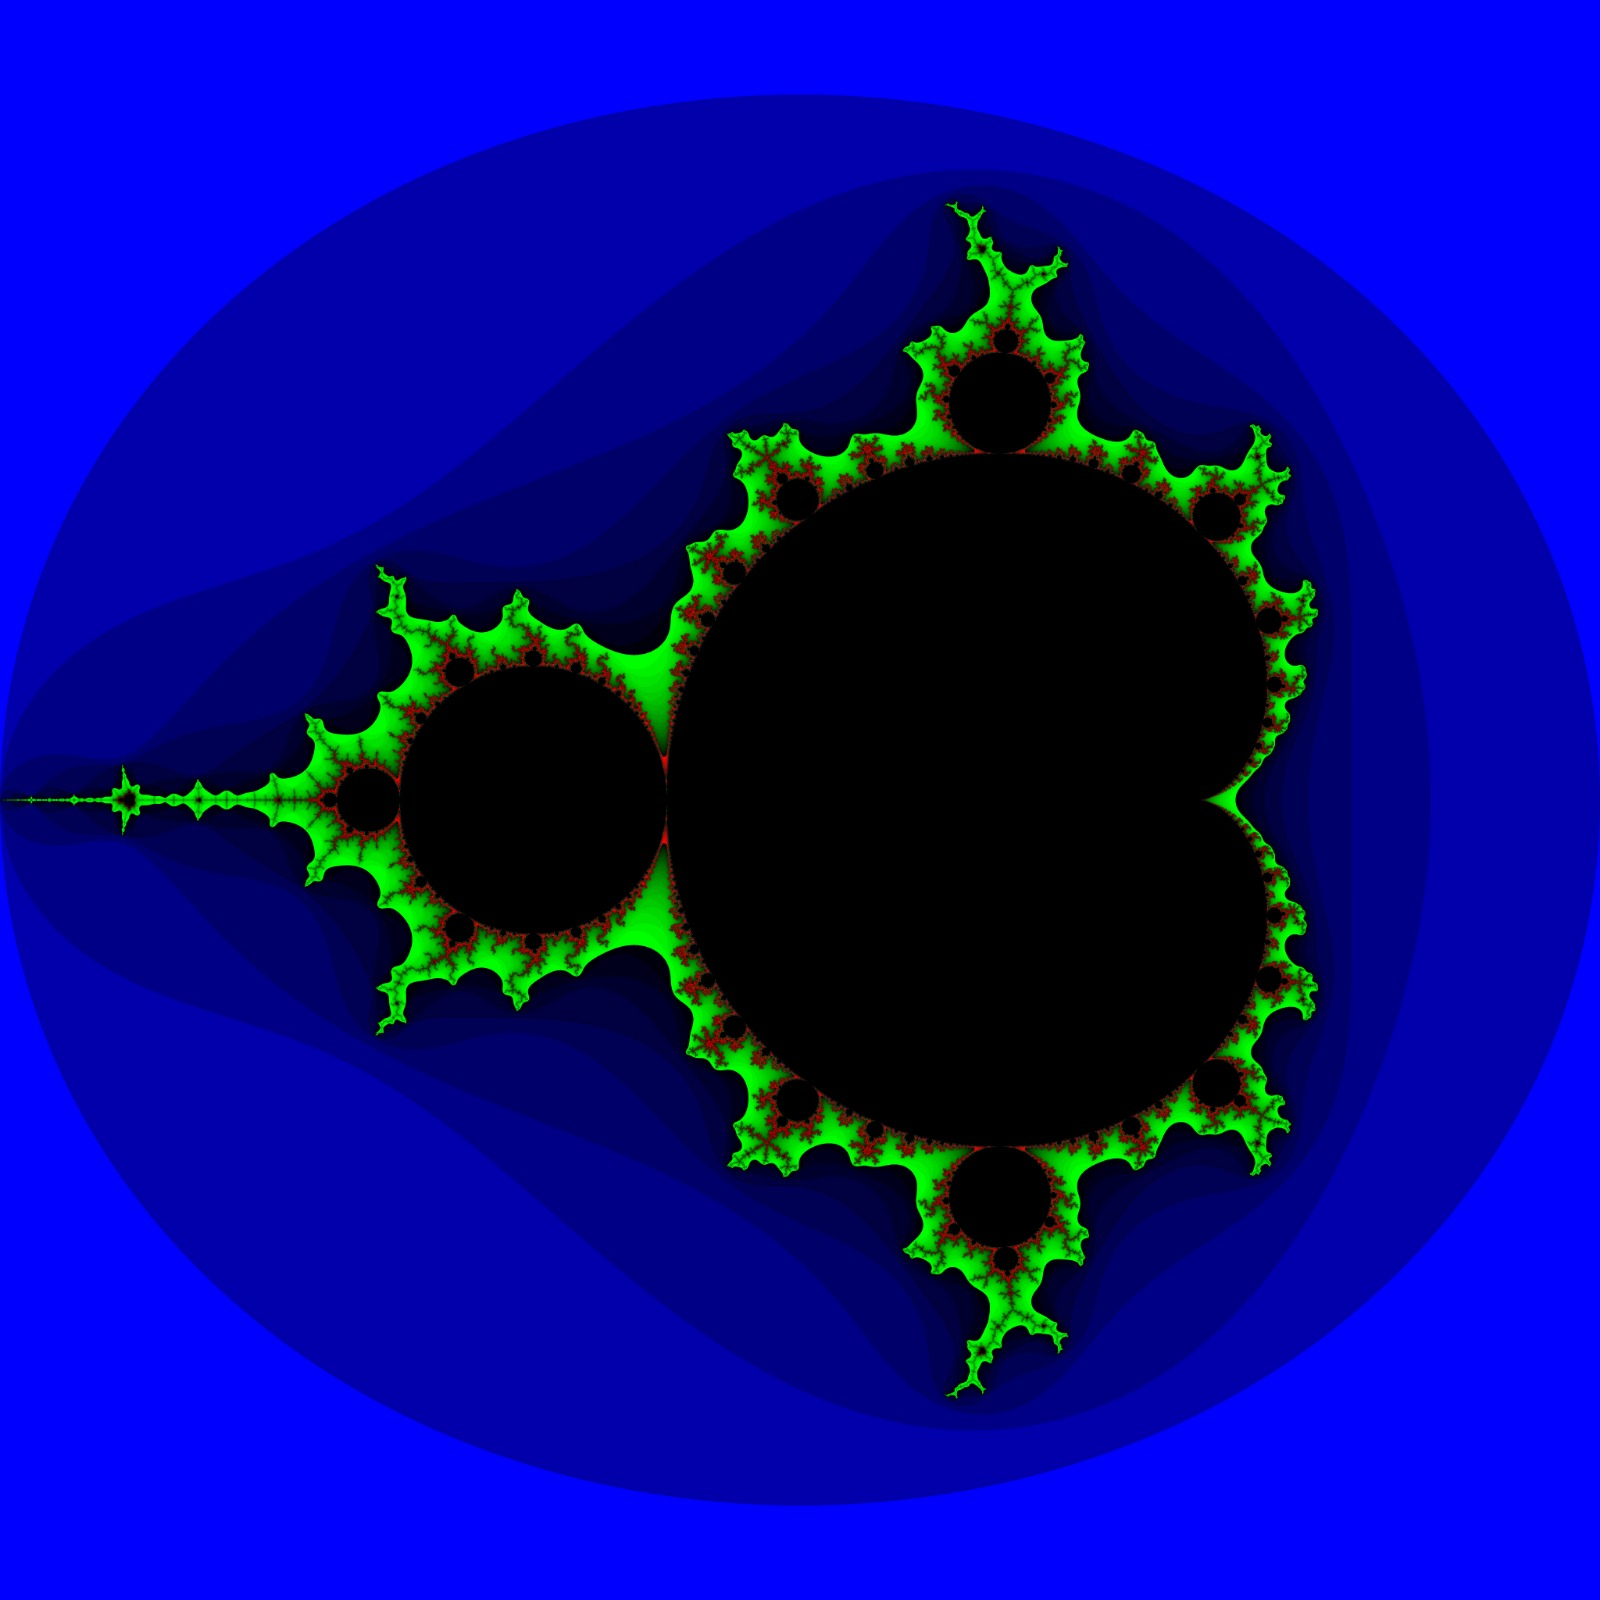
\includegraphics[scale=0.17]{mandelbrot.jpg}
    \caption{The Mandelbrot set colored with escape time algorithm}
    \label{comms}
\end{figure}
\newpage
\noindent
There are three tabulated data tables for the resolutions mentioned previously. They depict the block size, the run-time of each program, and the speedup ratios.\\\\
In the tables below it is shown that as the problem size increases, speedup increases meaning that GPU implementation is more beneficial when the problem size is large. Also it should be noted that the maximum allowable block size in Colab is 32x32 and it is used in the analyses. 

% Table for 2048x2048
\begin{table}[h]
\centering
\caption{Performance for Problem Size 2048x2048 and Block Size 32x32}
\label{tab:2}
\begin{tabular}{@{} ccc @{}}
\toprule
Time Taken (s) & Time Taken (s) & \\
Serial & CUDA & Speedup\\
\midrule
3.625 & 0.169 & 21.5 \\
\bottomrule
\end{tabular}
\end{table}

% Table for 4096x4096
\begin{table}[h]
\centering
\caption{Performance for Problem Size 4096x4096 and Block Size 32x32}
\label{tab:3}
\begin{tabular}{@{} ccc @{}}
\toprule
Time Taken (s) & Time Taken (s) & \\
Serial & CUDA & Speedup\\
\midrule
14.508 & 0.423 & 34 \\
\bottomrule
\end{tabular}
\end{table}

% Table for 8192x8192
\begin{table}[htbp]
\centering
\caption{Performance for Problem Size 8192x8192 and Block Size 32x32}
\label{tab:4}
\begin{tabular}{@{} ccc @{}}
\toprule
Time Taken (s) & Time Taken (s) & \\
Serial & CUDA & Speedup\\
\midrule
58.196 & 1.38 & 42 \\
\bottomrule
\end{tabular}
\end{table}




%%%%%%%%%%%%%%%%%
\clearpage

\section{Conclusion}
In the project, the GPU Tesla T4's cores are utilized for the parallelization of a Mandelbrot function and the results are compared with the serial approach. The speedup ratios are also presented in the tables Table \ref{tab:2}, Table \ref{tab:3}, and Table \ref{tab:4}. Results show that the parallelization significantly reduces the runtime when compared with the serial code.\\\\
\noindent
In the previous works, several implementations for computational mechanics that initialized MPI were compared with their serial versions. Although those implementations were more complicated than the implementations presented in this report, the increase in speed-up is nowhere near CUDA acceleration. The correct implementation of CUDA is very beneficial and should be encouraged. However, it is common knowledge that the memory copying between GPU to CPU take time, and should be a major consideration for the application of CUDA. For the problem of this report, the entirety of computations are made on CUDA and the results are copied to the device.\\\\
\noindent
In conclusion, when one wants to use GPU parallelization over MPI, the vital part of the parallelization is to distribute the workload among multiple processes as there are thousands of "workers" available to us. The choice of the block size is critical, as having too few may lead under-utilization of the GPU while too many may result in overhead. Another point is that GPUs often are more advantageous for parallel tasks, resulting more operations per second per watt of power compared to CPUs. This makes GPUs a more energy-efficient choice for tasks that can leverage their parallel processing capabilities, even though their absolute power consumption might be higher [3].
\noindent

\newpage
\section{References}

[1] Lecture notes of Ali Karakuş for ME489 (2023).
\\
\newline
[2] \text{https://www.techpowerup.com/gpu-specs/tesla-t4.c3316}
\\
\newline
[3] \text{https://www.icdrex.com/cpu-vs-gpu-which-one-is-right-for-your-workload/}

\end{document}